\documentclass{article}
\usepackage{biblatex}
\usepackage[utf8]{inputenc}
\usepackage[]{graphicx}
\usepackage{subfig}
\usepackage{blindtext}
\usepackage{amsmath}
\usepackage[margin=1in,bindingoffset=15.5mm,heightrounded]{geometry}
\usepackage{float}
\usepackage{blindtext}
\usepackage{appendix}
\usepackage[framed,numbered,autolinebreaks,useliterate]{mcode}
\addbibresource{source.bib}
\title{Simplifying Breast Cancer Interaction Network ODEs}
\author{Gabriel Wies and Connor White}
\date{May 2022}

\begin{document}

\maketitle

\section{Introduction}
Many biological phenomena, such as rare diseases, can be investigated through the use of applied scientific computing methods. Numerical analysis through applied scientific computing is very useful when looking at large models with many parameters and equations. The article “A Mathematical Model of Breast Tumor Progression Based on Immune Infiltration” in the Journal of Personalized Medicine, utilizes this approach to examine tumor progression in breast cancer patients with varying immune profiles by creating a model of ordinary differential equations (ODEs).

We created a simplified mathematical model of breast cancer tumor growth based on immune system status by adapting the model created in the previously mentioned article. The model presented uses a system of ODEs that models the growth and decay of 11 cell types and 6 molecules within the tumor. In order to simplify the system, variables that converge quickly to their steady-state in the original model will be replaced with constants. $T_N$, $T_h$, $T_r$, $D$, $M_N$, $M$, and $E$ all appear to converge quickly based on figure 5 in the article. The equations for $T_C$, $D_N$, $C$, $N$, $A$, $H$, $IL_{12}$, $IL_{10}$, $I_{\gamma}$, and $IL_6$ can be simplified heavily by replacing applicable variables with constants.

In the article there are 5 different clusters of data collected to observe immune cell frequencies in each cluster’s environment. In order to simplify the model further, only cluster 4 was simulated in our analysis. Results for all variable dynamics were obtained using an ODE solver in MATLAB, such as \mcode{ode45}, \mcode{ode113}, or \mcode{ode78}. The appropriate solver method was chosen based on the problem type (level of stiffness), accuracy, and computational efficiency. Results of the simplified simulation were compared to the original article to measure the efficacy of our simplified mathematical model. Using different combinations of constants in place of variables and manipulating set values also allowed us to understand the significance of the different estimated variables in the model, as well as the inner workings between the variables \cite[]{jpm11101031}.


\section{Methods}
\subsection{Model Formulation}
\subsubsection{Cluster Selection}
For simplicity, the model used the parameters, initial values, and steady state values from cluster 4. Clusters 1 and 4 have a higher percentage of aggressive sub-types of tumors than clusters 2,3, and 5. Cluster 4 was chosen over 1 due to the lower growth rate of Cluster 4. 
\subsubsection{Equation Selection and Formulation}
\paragraph{Non-dimensionalization}
The Simplified ODE system is based on the non-dimensionalized formulas provided on pages 26 and 27 of the article. The initial values of the dimensional variables were converted into non-dimensional values by solving $\left[\bar{X}\right] = \frac{\left[X\right]}{X^{\infty}} $. Non-dimensionalizing the ODEs allows for equations that converge quickly to be set equal to 1 in the simplified model. Non-dimensionalizing also allows for more stable numerical simulations. 

Setting $T_N$, $Th$, $Tr$, $D$, $M_N$, $M$, and $E$ to their steady state values results in all instances of these variables in the non-dimensionalized ODE equalling 1. Parameters were not non-dimensionalized with respect to time so the production and decay rates of the cells and molecules with respect to time were left unchanged. The simplified and non-dimensionalized system of ODEs contains 10 equations and 10 variables (appendix \ref{appendix:ODE}). The non-dimensional parameters for these equations were extracted from table A4 of the article (appendix \ref{Table A4}). The simplified ODE system was then input into MATLAB for simulation.

\subsection{ODE Solver Selection}
\subsubsection{ODE Properties}
When choosing an ODE solver to use in MATLAB it is important to take into account the properties of the ODE. One of the properties of an ODE is the problem type, which pertains to the stiffness of the ODE, and can fall under the category of stiff, nonstiff, or fully implicit. Stiffness is difficult to quantify, so in order to determine the problem type of our ODE we tried using different solver methods to compare their efficiency: \mcode{ode45} as a nonstiff solver and \mcode{ode15s} as a stiff solver. To compare the efficiency we measured the computation time MATLAB took to solve the ODE with each solver by using the \mcode{tic} and \mcode{toc} functions, and found that on average \mcode{ode45} took ~1.3 seconds and ODE15s took ~0.2 seconds to complete. Since \mcode{ode15s} is the more efficient solver we determined that our ODE is more stiff than nonstiff, however we wanted to take accuracy into account as well.

\subsubsection{Accuracy and Efficiency}
The different ODE solvers in MATLAB have varying levels of accuracy ranging from low to high. \mcode{ode15s} has low to medium accuracy and the rest of the stiff solvers have low accuracy, \mcode{ode45} has medium accuracy and there are other nonstiff solvers with improved accuracy: \mcode{ode113} has low to high accuracy, and \mcode{ode78} and \mcode{ode89} both have high accuracy. Since we are creating a simplified version of the model in the article, we determined that accuracy is the most important aspect for our model because one of our objectives is to emulate the cell and molecule behavior from the original model \cite{MAT}. 

The difference in computation time of ~1 second between stiff and nonstiff solvers is not significant for our analysis since we are only looking at one cluster of data and performing the simulation for a limited number of times. For a more robust model such as the original, using a stiff solver to reduce computation time would provide much more value since the simulation has to be repeated for each cluster.  Given this difference in scale, we decided to prioritize accuracy over efficiency. When testing \mcode{ode15s} compared to \mcode{ode45} we found that the latter mirrored the results from the article more closely, which makes sense given that \mcode{ode15s} has low to medium accuracy compared to \mcode{ode45}’s medium accuracy. We decided to prioritize accuracy since the efficiency of the nonstiff solvers is insignificant to that of the stiff solvers for the scope of our model. We then tested \mcode{ode113}, \mcode{ode78}, and \mcode{ode89} to compare their efficacy to \mcode{ode45}. Using the same methodology, we measured the efficiency of the solvers and found that \mcode{ode113} took ~3.3 seconds, \mcode{ode78} took ~2.7 seconds, and \mcode{ode89} took ~4.2 seconds. All of these solvers took at least twice the amount of time that \mcode{ode45} took and we observed that all of their solutions equally mirrored the solutions from the article. Since \mcode{ode45} was equally accurate to the other nonstiff methods but at least twice as efficient and more accurate than \mcode{ode15s}, we decided to select \mcode{ode45} as the best solver for the scope of our model \cite{MAT}.

\subsection{Shifting Parameters}
After selecting our ODE solver method, we determined which parameters we could shift in order to produce changes in our results. More specifically, we wanted to focus on the changes in relative tumor size and cancer cell proliferation when certain parameters were shifted to determine their relationships. In order to do so we looked at the parameters in two groups: molecules and cells. The molecules in the model are: $H$, $IL_{12}$, $IL_{10}$, $E$, $I_\gamma$, and $IL_6$. The cells in the model are: $T_h$, $T_c$, $T_r$, $T_n$, $D$, $D_n$, $M$, $M_n$, $C$, $A$, and $N$. 

We first investigated the shifting of molecules by changing their initial values aggressively (e.g. setting the initial value to zero, doubling or quadrupling the values). Shifting these parameters produced practically insignificant changes in our results. Apart from changing the starting y-position, the graphs quickly converged to the same rate as when the parameters were at their original values. This behavior was consistent with all molecules and we observed no significant changes to any of the solutions, so we shifted our focus to the cell parameters.

Of the eleven cells in our model, six of them were estimated as constants and set to their steady state values: $T_N$ , $T_h$, $T_r$ , $D$, $M_N$ , $M$ (equal to 1 in non-dimensionalized model). To see if shifting the cell parameters would have a more significant effect, we made aggressive changes to their initial values similar to our approach for the molecules. From doing so we quickly saw changes in our results, so we decided to move forward with shifting the initial cell values at consistent specified intervals. To do this we made four more identical versions of our ODE function in MATLAB so we could have four parameter shifts and observe them all on the same plot compared to the normal result. The parameter shifts we chose were $+0.1$, $+0.5$, $-0.1$, and $-0.5$, and we applied the shifts to the same initial cell value in each of the four ODE functions and then repeated this process for all of the cells. We observed the behavior of our results from these parameter shifts for total relative tumor size and dynamics of cancer cells.

\section{Results}
\paragraph{Comparing Results}
Before shifting the parameters of our model we first ran the simulation with the given initial values and our specified constants. We did this in order to evaluate the efficacy of our simplified model compared to the original model from the article. For this evaluation we observed the convergences of each variable graph compared to the convergences from the graphs for the corresponding variables from the article (appendix \ref{appendix:graph}). For all of the variables our results had the same or very similar behavior to the results from the article, so we deemed our simplified model as a successful representation of the actual model. With this accuracy verified, we moved forward with the parameter shifts in order to observe their effects on tumor size and cancer dynamics. 
\subsection{Effects on Tumor Size}
Our results for relative tumor size are similar to the total cell count results in the article. For our model we have relative tumor size rather than actual cell count size due to the non-dimensionalization of our equations. A tumor size of 12 mirrors the non-dimensionalized steady state of the tumor. 

\begin{center}
\begin{figure}
\begin{tabular}{cc}
\subfloat{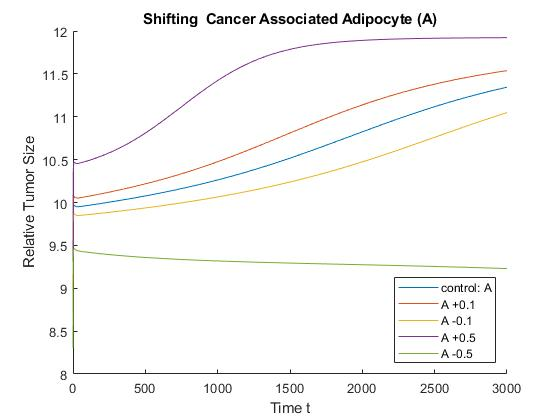
\includegraphics[width=6cm, height=4cm]{tumor/A.jpg}} &
\subfloat{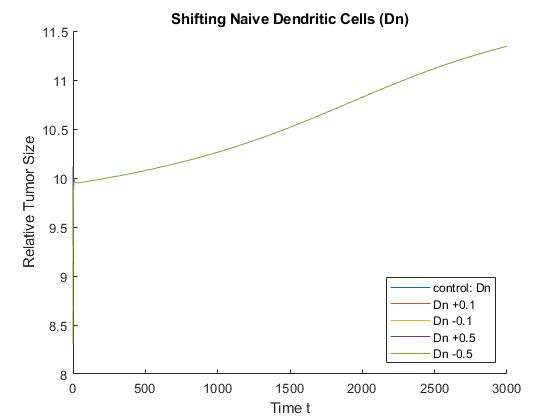
\includegraphics[width=6cm, height=4cm]{tumor/Dn.jpg}}\\
\subfloat{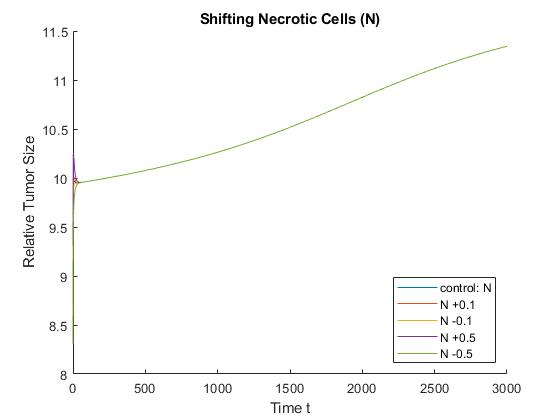
\includegraphics[width=6cm, height=4cm]{tumor/N.jpg}} &
\subfloat{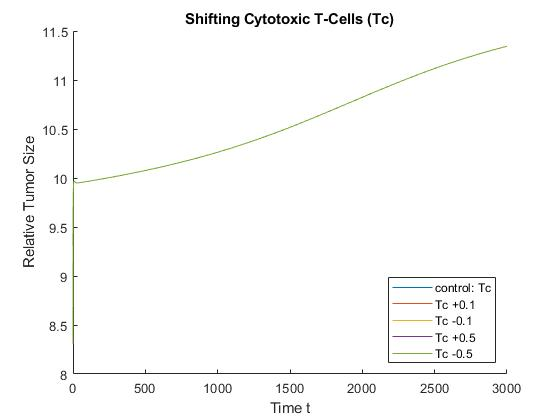
\includegraphics[width=6cm, height=4cm]{tumor/Tc.jpg}}\\
\end{tabular}
\caption{Tumor dynamics for shifting initial values of cells}
\begin{tabular}{cc}
\subfloat{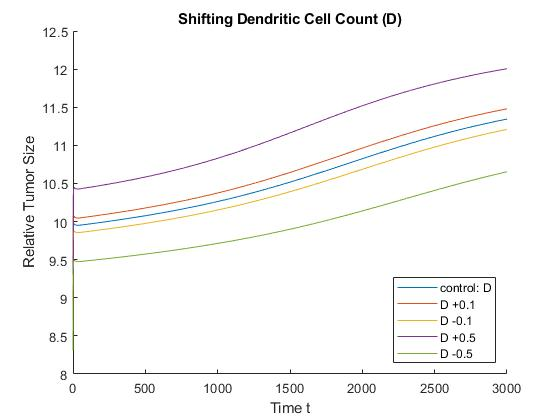
\includegraphics[width=6cm, height=4cm]{tumor/D.jpg}} &
\subfloat{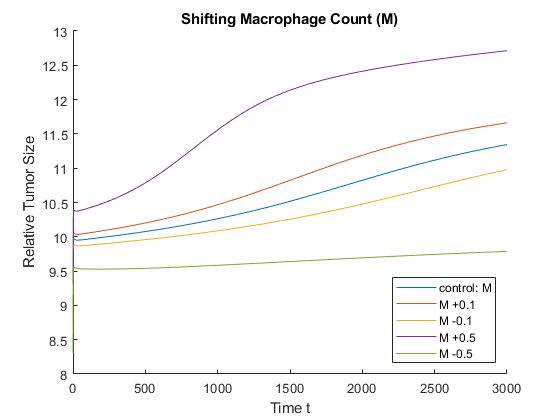
\includegraphics[width=6cm, height=4cm]{tumor/M.jpg}}\\
\subfloat{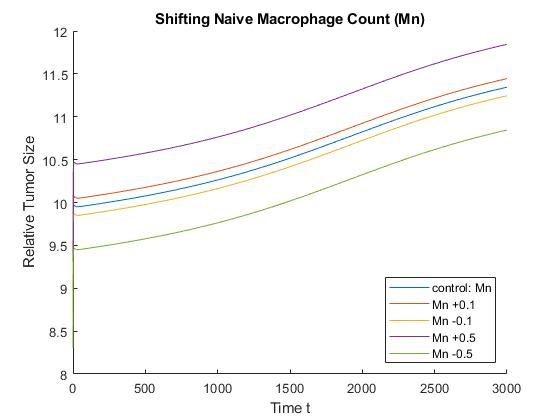
\includegraphics[width=6cm, height=4cm]{tumor/Mn.jpg}} &
\subfloat{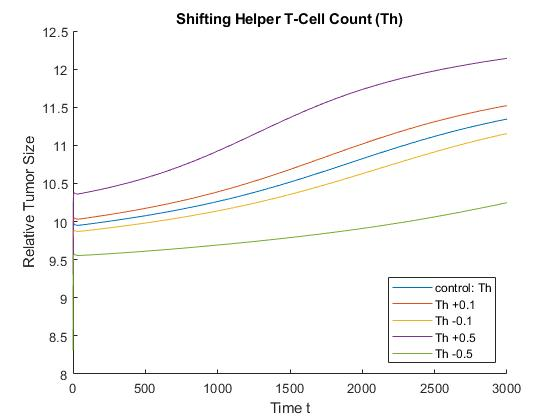
\includegraphics[width=6cm, height=4cm]{tumor/Th.jpg}}\\
\subfloat{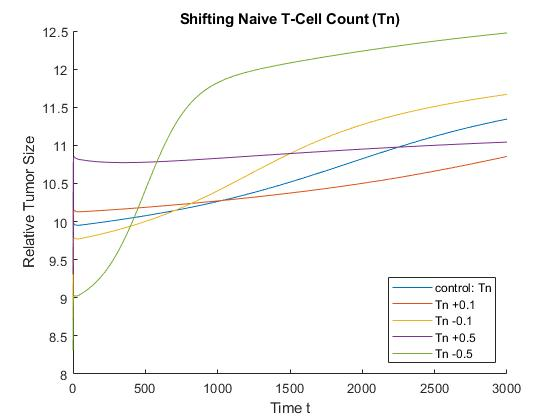
\includegraphics[width=6cm, height=4cm]{tumor/Tn.jpg}} &
\subfloat{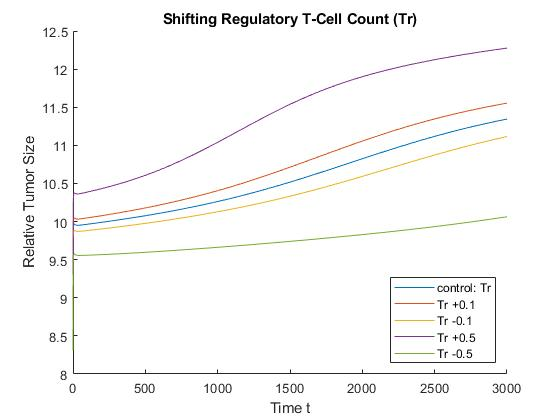
\includegraphics[width=6cm, height=4cm]{tumor/Tr.jpg}}\\
\end{tabular}
\caption{Tumor dynamics for shifting values of constants}
\end{figure}
\end{center}


\newpage

\subsubsection{Behavior}
We observed the effects of the parameter shifts for each variable on the total relative tumor size. The shifting of Naive Dendritic Cells ($D_n$), Necrotic Cells ($N$), and Cytotoxic T-Cells ($T_c$) all had a similarly insignificant effect on tumor size, in which the total relative tumor size remained the same as when these parameter shifts were not in place. The relative tumor size with no parameter shifts applied to it is denoted as the control line, which is used to compare to the relative tumor sizes with applied parameter shifts.

The shifting of dendritic cell count ($D$) and naive macrophage count ($M_n$) had a similar effect on tumor size. For the shift in Mn, the relative tumor size maintains the same slope and convergence rate as the control with the parameter shifts proportionally changing the y-intercepts. This shows that increasing or decreasing the initial naive macrophage count proportionally increases or decreases the relative tumor size, likely because we set $M_n$ to be a constant so a shift in $M_n$ causes the same relative shift in tumor size. For the shift in $D$, the relative tumor size has a similar proportional increase or decrease but as the shifted relative tumor sizes approach their steady state, the difference between the shifted sizes and control size increases. This difference is more noticeable in the +/-.5 parameter shifts than it is in the +/-.1 shifts, which leads us to the conclusion that the greater the shift in the initial count of Dendritic Cells the relative tumor size will either increase or decrease at a greater rate than that of shifting the initial Naive Macrophage count.

The shifting of helper T-cell count ($T_h$) and regulatory T-cell count ($T_r$) had a similar effect on tumor size and a similar behavior in growth to shifting $D$. As with shifting $D$, the greater the shift in $T_h$ or $T_r$ is, the greater the difference will be between the shifted relative tumor sizes and control sizes as they approach steady-state. Shifting $T_r$ causes a greater difference between shifted relative tumor sizes than that of $T_h$. Shifting Th results in a relatively proportional shifted tumor size, but a positive shift causes a greater increase in slope than a negative shift as the magnitude of the shift increases. $T_r$ behaves similarly in the sense that a positive shift causes a greater increase in slope than a negative shift of the same magnitude. The difference between the shifted relative tumor size and control size is greater for $T_r$ than it is for $T_h$. This leads us to conclude that shifting the initial value of $T_r$ has a more significant effect on relative tumor size growth than that of $T_h$.

As with $T_h$ and $T_r$, the shifting of macrophage count ($M$) and cancer associated adipocyte ($A$) causes the difference between the shifted relative tumor sizes and control sizes to grow with time. When $M$ is shifted +/-.1 the difference between the shifted relative tumor size and control size grows with time initially but around $t = 2000$ the difference appears to reach a constant level and the shifted relative tumor size and control size begin to grow at the same rate. For $A$, the difference between shifted relative tumor size and control size for +/-.1 grows with time initially but around $t = 2000$ the difference begins to decrease, showing that given enough time a +/-.1 shift in $A$ has less of an effect on relative tumor size than a +/-.1 shift in $M$. However, for a larger shift in $A$ such as +/-.5 the shifted relative tumor size behaves much differently. A shift in $A$ of +.5 causes the slope of the shifted relative tumor size to increase at a faster rate than that of $M$, and it converges to a flat rate within the time interval whereas $M$ still has a positive slope at the end of the time interval. For a -.5 shift in both $M$ and $A$, the difference between shifted relative tumor size and control size increases with time, but the shifted size of $M$ has a very small positive slope while the shifted size of $A$ has a negative slope. A positive shift in $M$ will cause the difference between shifted relative tumor size and control size to increase at a greater rate with time than that of $A$. A negative shift in $M$ will cause the shifted relative tumor size to increase at a lower rate with time than that of $A$. From this we can conclude that a positive or negative shift of $A$ results in a smaller relative tumor size than a positive or negative shift of $M$.

The shifting of naive T-cell count ($T_n$) has a unique effect on relative tumor size than the rest of our variables. A negative shift in $T_n$ causes relative tumor size to grow and a positive shift in $T_n$ causes relative tumor size to decrease, behaving inversely to our other variables. Shifting $T_n$ by +.1 results in a very small positive slope that eventually is overtaken by the control, and shifting by +.5 results in a larger positive slope that still results in the shifted relative tumor size being less than the control by the end of the time period. Shifting Tn by -.1 causes the shifted relative tumor size to behave inversely to that of the shift by +.1. Shifting $T_n$ by -.5 causes a large increase in relative tumor size at a sharp rate until around $t = 1000$, where it then continues to increase at a steady positive rate. This behavior of $T_n$ allows us to conclude that removing $T_n$ cells, or having lower than average levels, makes the risk of cancer tumor growth much greater. 



\subsection{Effects on Cancer Dynamics}
Our results for cancer cells are using the non-dimensionalized ODE system. As a result the values given are relative to the steady state of cancer cells in cluster 4 where 1 equals the steady state. 

\subsubsection{Behavior}
\subsubsection{Shifting Initial condition of variables}
The shifting of the initial values of Naive Dendritic Cells ($D_n$), Necrotic Cells ($N$), and Cytotoxic T-Cells ($T_c$) all had similarly insignificant effects on the amount of cancer cells ($C$). Shifting the initial values of Cancer Associated Adipocyte (A) had a significant impact on the amount of cancer cells. When $A$ was shifted up by .5, the growth rate of $C$ skyrocketed resulting in the near steady state of $C$ being achieved quickly. When the initial value of A was decreased by .5 it resulted in $C$ decreasing over time until it reached near zero. The relationship between $C$ and $A$ displayed in the simplified ODE system matches the interaction network displayed in Figure 1. of the article (appendix \ref{appendix:article}). 
\subsubsection{Shifting Constants}
Shifting the non-dimensionalized constant of naive macrophages ($M_n$) resulted in an insignificant change in the dynamics of  $C$. 
Shifting the values of helper t-cells ($T_h$) and regulatory t-cells ($T_r$) had similar effects on $C$. Decreasing these constants led to a decrease in the growth rate of $C$. The steady state value of $C$ decreased as  $T_h$ and $T_r$ decreased.  A more severe version of this relationship was displayed between Macrophages ($M$) and C. When the constant $M$ was increased, the growth rate of $C$ also increased. When $M$ was increased by .5, the predicted steady state of $C$ was well above 1. Decreasing $M$ by .5 resulted in $C$ reaching a steady state of nearly 0. While this relationship was not shown in the interaction network of the article, the network does show that an increase in $C$ also leads to an increase in $M$. 
Increasing the value of naive t-cells ($T_n$) led to a decrease in $C$. When $T_n$ was increased by .5, a steady state of 0 was achieved for $C$ quickly. When $T_n$ was decreased, the steady state value of $C$ was almost 2. This shows that $T_n$ play a huge role in the inhibition of tumor growth. 

\begin{center}
\begin{figure}
\begin{tabular}{cc}
\subfloat{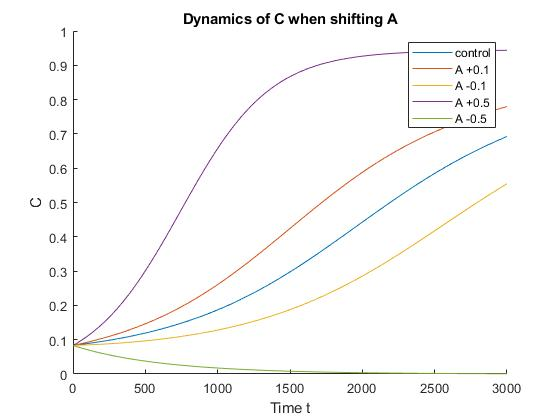
\includegraphics[width=6cm, height=4cm]{cancer/A.jpg}} &
\subfloat{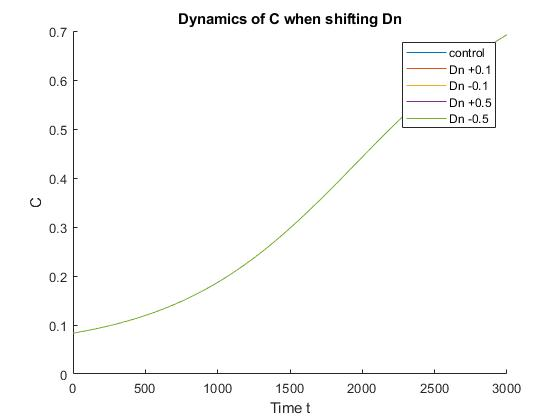
\includegraphics[width=6cm, height=4cm]{cancer/Dn.jpg}}\\
\subfloat{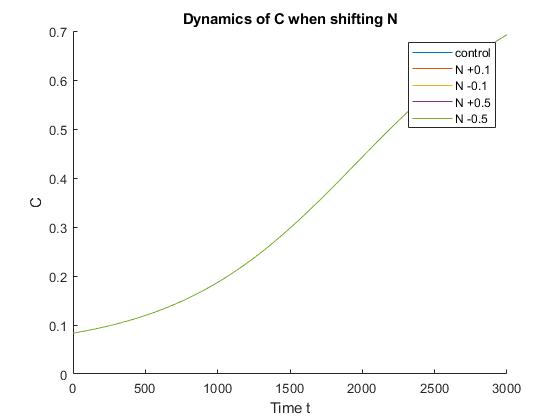
\includegraphics[width=6cm, height=4cm]{cancer/N.jpg}} &
\subfloat{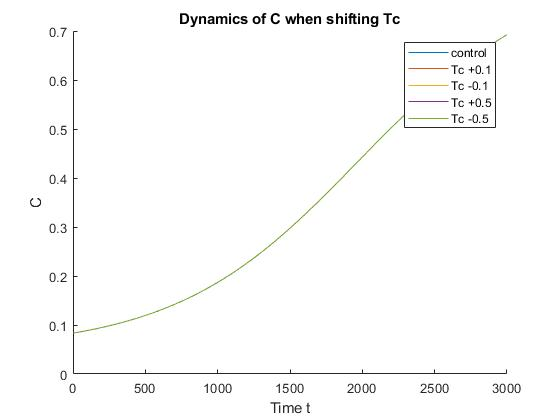
\includegraphics[width=6cm, height=4cm]{cancer/Tc.jpg}}\\
\end{tabular}
\caption{Cancer Cell dynamics for shifting initial values of cells}
\begin{tabular}{cc}
\subfloat{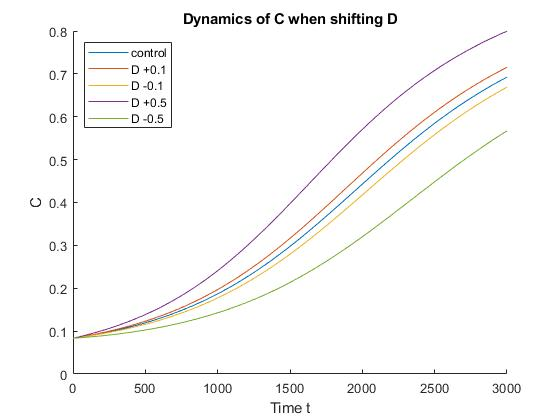
\includegraphics[width=6cm, height=4cm]{cancer/D.jpg}} &
\subfloat{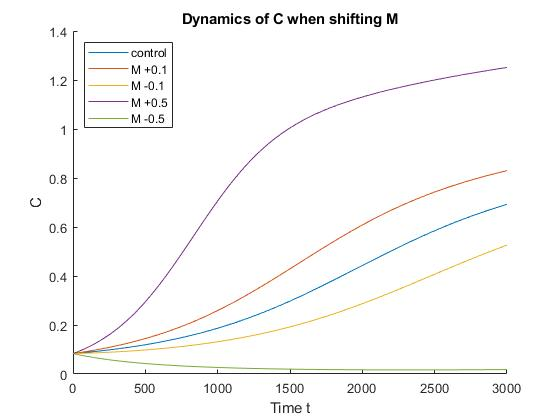
\includegraphics[width=6cm, height=4cm]{cancer/M.jpg}}\\
\subfloat{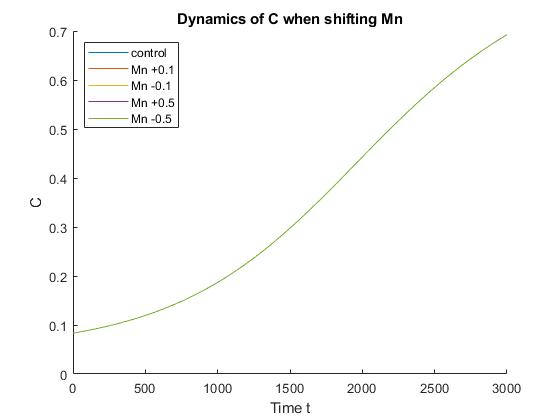
\includegraphics[width=6cm, height=4cm]{cancer/Mn.jpg}} &
\subfloat{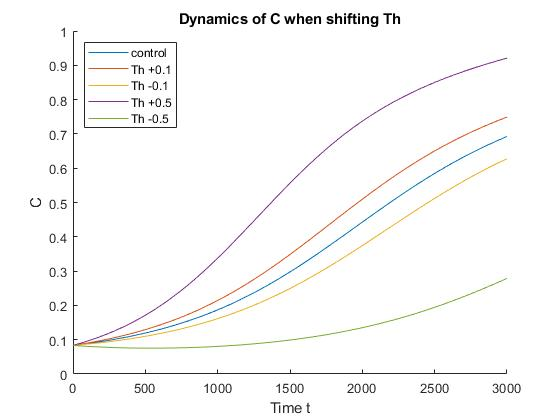
\includegraphics[width=6cm, height=4cm]{cancer/Th.jpg}}\\
\subfloat{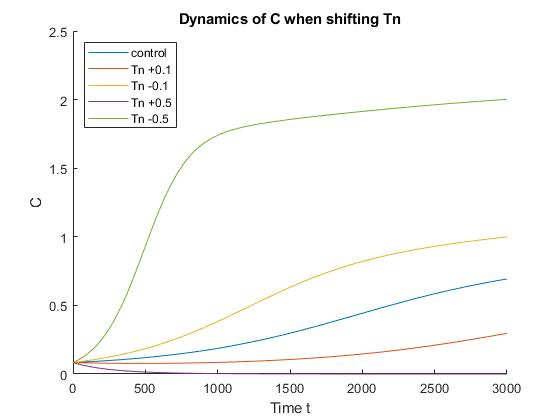
\includegraphics[width=6cm, height=4cm]{cancer/Tn.jpg}} &
\subfloat{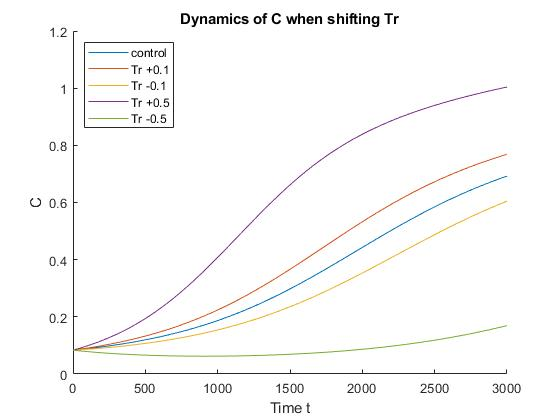
\includegraphics[width=6cm, height=4cm]{cancer/Tr.jpg}}\\
\end{tabular}
\caption{Cancer cell dynamics for shifting values of constants}
\end{figure}
\end{center}
\newpage
\section{Conclusion}
Shifting the parameters of the simplified ODE system did affirm the general interaction network presented in Figure 1. of the article (appendix \ref{appendix:article}), certain interactions were not preserved such as the relationship between dendritic cells and tumor cells. Data was lost with the simplification of the model, but general trends were preserved. While the simplified ODE system did produce satisfactory results for Cluster 4, we have yet to show that a similar method of simplification would work for the other clusters. It may also be the case that a better way to simplify the model could be discovered through looking at the other clusters.

\subsection{Next Steps}
A more accurate simplification of the ODE system in the article could potentially be produced if the system was reduced before non-dimensionalizing. Different $\bar{\lambda}$ and $\bar{\delta}$ values would be determined when compared to the values provided. This would require a more in depth understanding of the growth and decay rates in the ODE system. Sensitivity analysis could also be done on the parameters in order to see what is lost by simplifying the system. While simplifying the original ODEs did lead to a system which mimicked the original, changing certain parameters could lead to wildly different results than if those parameters were shifted in the original system. 
\newpage
\appendix 
\section{ODE}
\label{appendix:ODE}
Simplified ODE where $T_N$, $T_h$, $T_r$, $D$, $M_N$, $M$, and $E$ are constants (Set equal to $1$ when simulating the ODE from the article).
\begin{align}
    \frac{d[\bar{T}_c]}{dt} &= (\bar{\lambda}_{T_cE}[\bar{E}]+\bar{\lambda}_{T_cD}[\bar{D}]+\bar{\lambda}_{T_cIL_{12}}[\bar{IL}_{12}])[\bar{T}_N]-(\bar{\delta}_{T_cT_r}[\bar{T}_r]+\bar{\delta}_{T_cIL_{10}}[\bar{IL}_{10}]+\delta_{T_c})[\bar{T}_c]\\
    \frac{d[\bar{D}_N]}{dt} &= \bar{A}_{D_N}-(\bar{\lambda}_{DC}[\bar{C}]+\bar{\lambda}_{DH}[\bar{H}]+\bar{\lambda}_{DE}[\bar{E}])[\bar{D}_N]-\delta_{D_N}[\bar{D}]\\
    \frac{d[\bar{C}]}{dt} &= (\lambda_C+\bar{\lambda}_{CIL_6}[\bar{IL}_6]+\bar{\lambda}_{CA}[\bar{A}]\left(1-\frac{[\bar{C}]}{\bar{C}_0} \right)[\bar{C}]-(\bar{\delta}_{CT_c}[\bar{T}_c]+\bar{\delta}_{CI_\gamma}[\bar{I}_\gamma]+\delta_C)[\bar{C}]\\
    \frac{d[\bar{N}]}{dt} &= \bar{\alpha}_{NC}(\bar{\delta}_{CI_\gamma}[\bar{I}_\gamma]+\bar{\delta}_{CT_c}[\bar{T}_c]+\delta_c)[\bar{C}]-\delta_N[\bar{N}]\\
    \frac{d[\bar{A}]}{dt} &= \lambda_A[\bar{A}]\left(1-\frac{[\bar{A}]}{\bar{A}_0}\right)-\delta_A[\bar{A}]\\
    \frac{d[\bar{H}]}{dt} &=\bar{\lambda}_{HD}[\bar{D}]+\bar{\lambda}_{HN}[\bar{N}]+\bar{\lambda}_{HM}[\bar{M}]+\bar{\lambda}_{HT_c}[\bar{T}_c]+\bar{\lambda}_{HC}[\bar{C}]-\delta_H[\bar{H}]\\
    \frac{d[\bar{IL}_{12}]}{dt} &= \bar{\lambda}_{IL_{12}M}[\bar{M}]+\bar{\lambda}_{IL_{12}D}[\bar{D}]+\bar{\lambda}_{IL_{12}T_h}[\bar{T}_h]+\bar{\lambda}_{IL_{12}T_c}[\bar{T}_c]-\delta_{IL_{12}}[\bar{IL}_{12}]\\
    \frac{d[\bar{I}_\gamma]}{dt} &= \bar{\lambda}_{I_{\gamma}T_c}[\bar{T}_c]+\bar{\lambda}_{I_{\gamma}T_h}[\bar{T}_h]+\bar{\lambda}_{I_{\gamma}D}[\bar{E}][\bar{D}]-\delta_{IL_6}[\bar{IL_6}]\\
    \frac{d[\bar{IL}_6}{dt} &= \bar{\lambda}_{IL_6A}[\bar{A}]+\bar{\lambda}_{IL_6M}[\bar{M}]+\bar{\lambda}_{IL_6D}[\bar{D}]-\delta_{IL_6}[\bar{IL}_6]
     \end{align}
     \begin{equation}
    \begin{aligned}
    \frac{d[\bar{IL}_{10}]}{dt} &=\bar{\lambda}_{IL_{10}M}[\bar{M}]+\bar{\lambda}_{IL_{10}D}[\bar{D}]+\bar{\lambda}_{IL_{10}T_r}[\bar{T}_r]+\bar{\lambda}_{IL_{10}T_h}[\bar{T}_h]+\bar{\lambda}_{IL_{10}T_c}[\bar{T}_c]+\bar{\lambda}_{IL_{10}C}[\bar{C}]\\
    &-\delta_{IL_{10}}[\bar{IL}_{10}]
    \end{aligned}
     \end{equation}
\newpage
\section{Comparing Results}
\label{appendix:graph}
Comparison between simplified ODE system(Left) and original ODE system from the article(Right). Note: The Black Line is cluster 4.\\
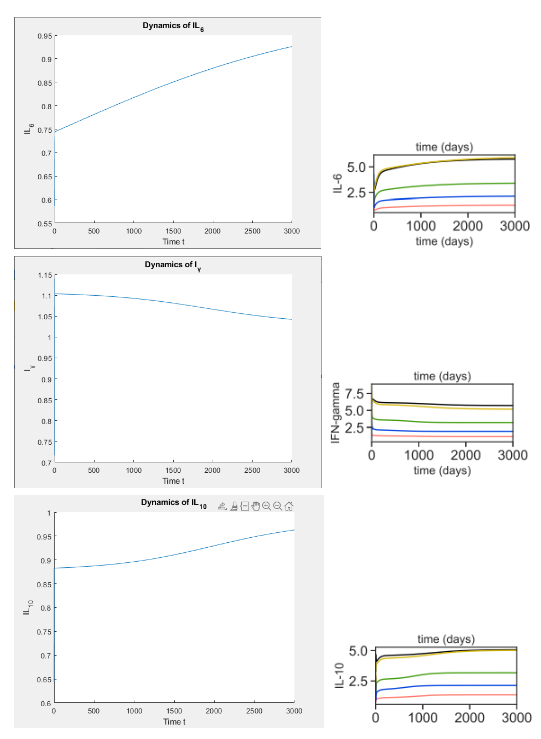
\includegraphics[]{comp1.PNG}\\
\newpage
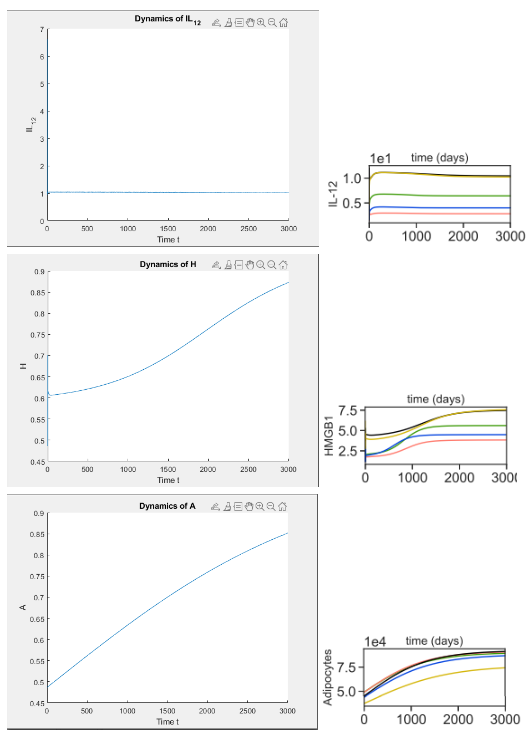
\includegraphics[]{comp2.PNG}\\
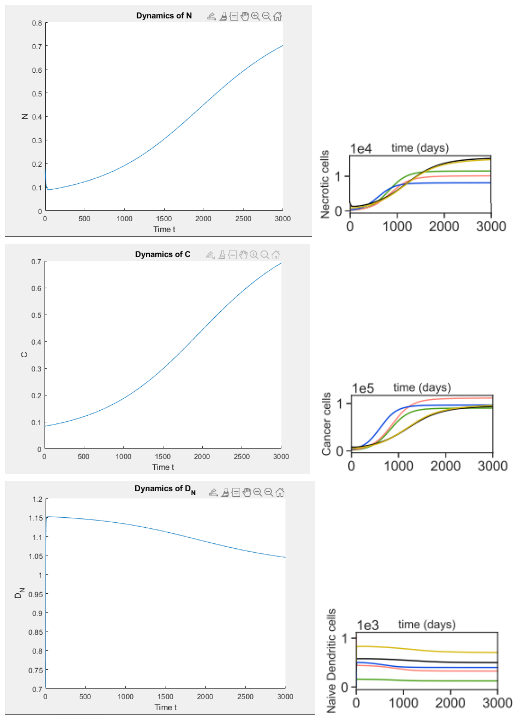
\includegraphics[]{comp3.PNG}\\
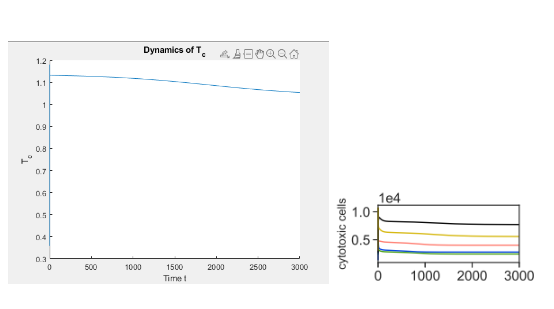
\includegraphics[]{comp4.PNG}\\
\section{Code}
\label{appendix:code}
MATLAB code for simplified ODE system
\begin{lstlisting}
function dydt = odefun1(t,y)

dydt = zeros(10,1);
T_n = 1;
T_h = 1;
T_r = 1;
D = 1;
M_n = 1;
M = 1;
E = 1;
%CD4+ Helpter T-Cells (Tc)
dydt(1) = (8.420*E + D*6.064e-3 + y(7)*3.95e-2)*T_n-(1.146*T_r+6.913*y(8)+.231)*y(1);
%Naive Dendritic Cells (DN)
dydt(2)  = 6.161e-1 -(2.540e-2*y(3)+1.474e-1*y(6)+1.663e-1*E)*y(2)-.277*y(2);
%Cancer Cells (C)
dydt(3)  = ((3.427e-2 + 5.530e-3*y(10) + 1.807e-3*y(5))*(1 - (y(3)/8.923))*y(3)) - ((8.052e-3*y(1) + 2.832e-3*y(9) + 2.606e-2)*y(3));
%Necrotic Cells (N)
dydt(4)  = (3.089*(2.832e-3*y(9) + 8.052e-3*y(1) + 2.606e-2)*y(3)) - 1.141e-1*y(4); 
%Cancer Associated Adipocytes (A)
dydt(5)  = (3.400e-3*y(5)*(1 - (y(5)/5.666))) - 2.8e-3*y(5); 
%HMGB1 (H)
dydt(6)  = 1.239*D + 3.552*y(4) + 7.101e-1*M + 7.244*y(1) + 5.255*y(3) - 18*y(6);
%IL-12(IL12)
dydt(7)  = 3.738e1*M + 6.521*D + 4.596e1*T_h + 3.813e1*y(1) - 128*y(7);
%IL-10(IL10)
dydt(8)  = 9.978e-1*M + 1.741e-1*D + 4.651e-1*T_r + 1.227*T_h + 1.018*y(1) + 7.384e-1*y(3) - 4.62*y(8);
%%IFN-gamma (Igamma)
dydt(9) = 2.611e1*y(1) + 6.295*T_h + 8.931e-1*E*D - 33.3*y(9);
%%IL-6 (IL6)
dydt(10)  = 5.329e-1*y(5) + 4.573e-1*M + 7.977e-2*D - 1.07*y(10);

end
\end{lstlisting}
MATLAB code for converting initial values to work in non-dimensionalized ODE and solving ODE system.
\begin{lstlisting}
tspan1 = [0 3000]; %time interval
y_0 = [2.76e3,3.51e2,7.96e3,2.71e3,4.49e4,5.29,6.88,3.27,4.10,3.40]; %control
% y0  = [Tc,    DN,    C,     N,     A,     H,   IL12, IL10,I-gamma, IL6]
%steady state values
y_ss = [7.71e3,4.99e2,9.54e4,1.54e4,9.22e4,7.54,1.04,5.08,5.72,5.80];
%convert y_0 into nondimn. values
y_0_bar = y_0_1./y_ss;
[t,y] = ode45(@odefun1,tspan1,y_0_bar);
\end{lstlisting}
\section{Original Article References}
\label{appendix:article}
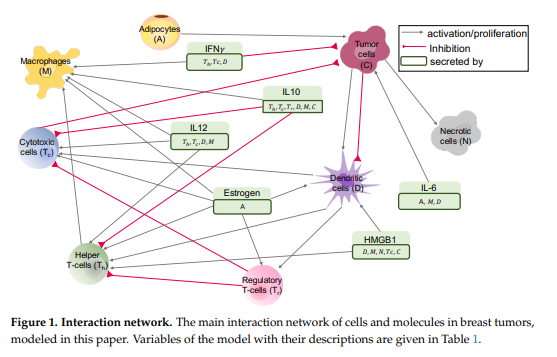
\includegraphics[scale=.75]{fig5.PNG}\\
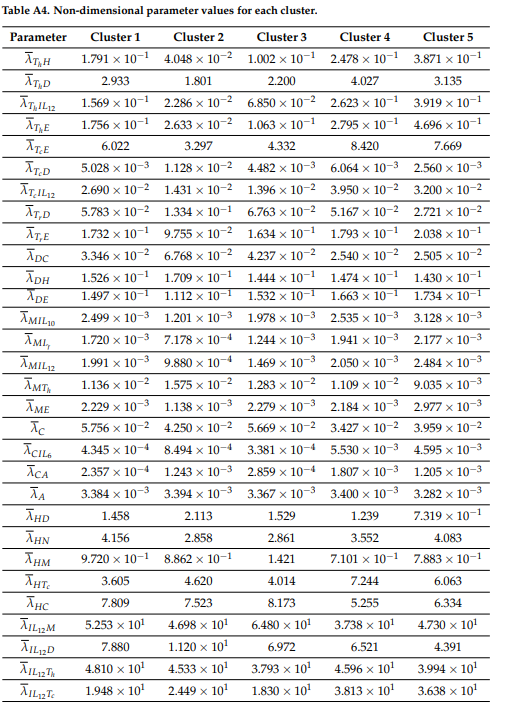
\includegraphics[scale=.75]{a4.PNG}\label{Table A4}\\
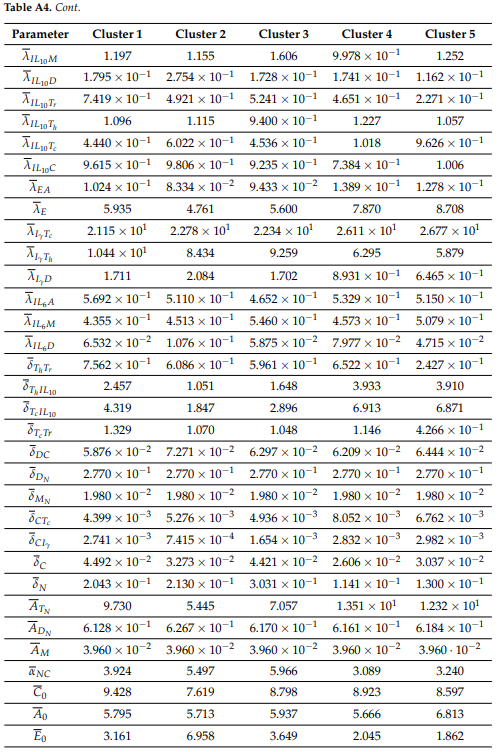
\includegraphics[scale=.75]{a42.PNG}
\printbibliography
\end{document}
